
\chapter{Transitie technieken}
\label{ch:h3}

Als men spreekt over het overschakelen naar IPv6, dan is het niet de bedoeling IPv4 direct aan de kant te leggen en volledig niet meer te gebruiken. Alleen een IPv6 netwerk is meestal niet het beste idee omdat niet iedereen een diepe kennis hiervan heeft. Daarom zou het beter zijn om eerst kennis te maken met IPv6 door gebruik te maken van beide protocollen. Het probleem is dat een IPv6 netwerk niet direct kan communiceren met een IPv4. Daarom zullen er verder in dit hoofdstuk enkele methodes worden besproken over hoe IPv6 nodes met IPv4 nodes kunnen communiceren via tunneling en inkapseling en translatie. Daarbij gaan we ook het beste scenario aantonen die ideaal zou zijn om aan de slag mee te gaan in een lokaal netwerk.

\section{Tunneling en inkapseling}

Om het connecteren van IPv6 hosts over een IPv4 netwerk, zal er gebruik gemaakt worden van een IPv6 tunnel over het IPv4 netwerk.

Het IPv6 pakket dat afkomstig is van het IPv6 apparaat van de verzender zal ingekapseld worden bij het toegangspunt van de tunnel, waar het een extra IPv4 header krijgt en vervolgens als IPv4 pakket zal verstuurd worden door het IPv4 netwerk. Bij het einde van de tunnel zal de IPv4 header verwijderd worden en het pakket zal nadien als een IPv6 pakket toekomen bij het IPv6 bestemmingsapparaat. Enkele methodes die verder worden uitgelegd zijn 6in4, 6to4, 6rd, GRE, ISATAP en DS-Lite \autocite{RIPE2016}.

\begin{figure}
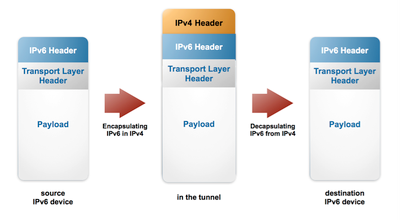
\includegraphics[width=\textwidth,height=\textheight,keepaspectratio]{Tunneling.png}
\centering
\caption{Tunneling en inkapseling \autocite{RIPE2016}}
\centering
\end{figure}

\subsection{6in4}

Als een IPv4 host, een IPv6 wilt bereiken maar geen ipv6 connectiviteit heeft thuis , is er de mogelijkheid een  6in4 tunnel op te zetten. Op het moment dat een IPv4 host een webserver via IPv6 wil bereiken is dit echter niet mogelijk. Hiervoor kan er gebruik gemaakt worden van een 6in4 tunnel. De host dient een tunnel op te zetten en gebruik te maken van een tunnelbroker. Via de tunnelbroker zal er een IPv6 adres beschikbaar zijn waarnaar de IPv6 pakketten verstuurd zullen worden. Een 6in4 tunnel zal een verzonden IPv6 pakket van de host omzetten naar een IPv4 pakket. Men zal een nieuwe IPv4 header toevoegen over de IPv6 header. Hierdoor kan het pakket verzonden worden over het IPv4 internet. Als het pakket de tunnelbroker bereikt dan zal hij op zijn moment het pakket uitpakken en de IPv4 header verwijderen. Nadien blijft enkel het oorspronkelijke IPv6 pakket over en wordt deze over het IPv6 internet verstuurd naar de webserver. Dit mechanisme is een stabiele en voorspelbare manier omdat men steeds weet naar waar het pakket zal verzonden worden. Voor een ISP is dit echter geen gangbare methode. Als een ISP gebruik zal maken van een 6in4 tunnel, dan zal deze voor iedere klant manueel een tunnel moeten aanmaken \autocite{RIPE2016}. 

\begin{figure}
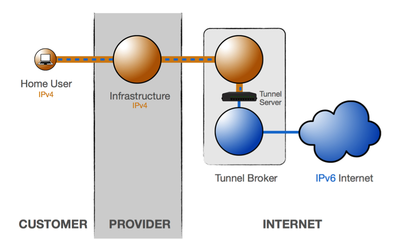
\includegraphics[width=\textwidth,height=\textheight,keepaspectratio]{6in4.png}
\centering
\caption{6in4 visualisatie \autocite{RIPE2016}}
\centering
\end{figure}

\subsection{6to4}

Doorgaans wordt 6to4 tunneling niet meer gebruikt. 6to4 is een tunneltechniek die het nadeel van de vorige mechaniek oplost, 6in4. Deze techniek is, in vergelijking met 6in4, beter schaalbaar op grotere vlakken. Hiermee zou een ISP voor al zijn klanten de techniek kunnen hanteren. Echter heeft deze methode enkele nadelen. Er kunnen zich op onverwachte momenten een lange latency veroorzaken met zeer negatieve gebruikservaringen tot gevolg. 6to4 gebruikt overal in de wereld dezelfde IPv6 en IPv4 prefix voor het begin en einde van de tunnel. Namelijk 2002::/16 voor IPv6 en 192.88.99.0/24 voor IPv4. Wanneer IPv6 bronapparaat met 6to4 tunnel een connectie wilt aangaan met een ander IPv6 apparaat over IPv4 internet, dan zal de tunnel automatisch een einde vinden zonder dat er configuratie nodig is aan de tunnel zelf. Hierdoor is de schaalbaarheid groot en dient er geen manuele configuratie meer te gebeuren. Echter heeft de eindgebruiker wel een publiek IPv4 adres nodig om de connectie succesvol tot stand te brengen. Het IPv4 tunneluitgangspunt is geïntegreerd in de bitnummers 17-48 van het 6to4 IPv6-adres. Dus het tunnelingangspunt neemt automatisch het IPv4-adres van het tunneluitgangspunt van de tunnel over van het IPv6-aders van de bestemming \autocite{RIPE2016}.

\begin{figure}
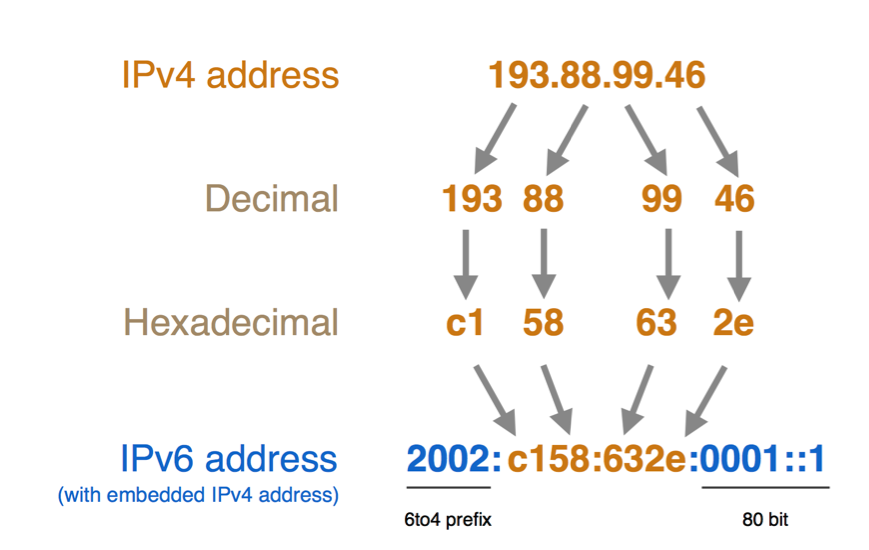
\includegraphics[width=\textwidth,height=\textheight,keepaspectratio]{6to4.png}
\centering
\caption{6to4 omzetting \autocite{RIPE2016}}
\centering
\end{figure}

Een schematische voorstelling van de verschillende delen van een 6to4 IPv6 adres is als volgt.

\begin{figure}
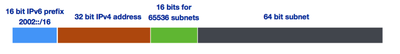
\includegraphics[width=\textwidth,height=\textheight,keepaspectratio]{6to4_2.png}
\centering
\caption{6to4 schematische voorstelling \autocite{RIPE2016}}
\centering
\end{figure}

Omdat de eindpunten van de tunnel anycasted zijn, wilt dit zeggen dat de gebruiker geen controle heeft over welke tunnel effectief gebruikt zal worden. Het terugkerende verkeer kan hierdoor ook een ander ingangspunt van een tunnel nemen wat kan leiden tot asymmetrische routes, lange latencies en onaanvaardbare wachttijden voor de gebruikers hiervan \autocite{RIPE2016}.

\begin{figure}
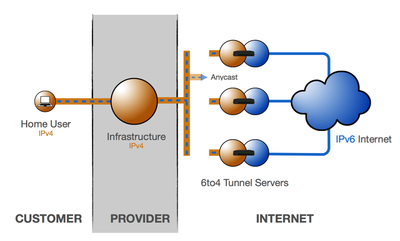
\includegraphics[width=\textwidth,height=\textheight,keepaspectratio]{6to4_3.png}
\centering
\caption{6to4 visualisatie \autocite{RIPE2016}}
\centering
\end{figure}

\subsection{6rd}

De derde methode namelijk 6rd, werd ontwikkeld om de problemen zoals lange latencies, die eigenaardig waren bij de tunneltechniek 6to4, op te lossen. Ook zal 6rd de schaalbaarheid behouden die te vinden was bij 6to4. Ondertussen is 6rd al ingevoerd bij enkele miljoenen personen \autocite{RIPE2016}. 

Het principe achter deze techniek is zeer eigenaardig aan die van 6to4. Eén van de belangrijkste verschillen is dat de IPv4 en IPv6 adresruimte van de ISP nu gebruikt zal worden voor de eindpunten van de tunnels. Dit betekent dat anycast niet langer meer gebruikt zal worden. Het verkeer wordt hierdoor symmetrisch en wordt door de ISP beheerd \autocite{RIPE2016}.

\begin{figure}
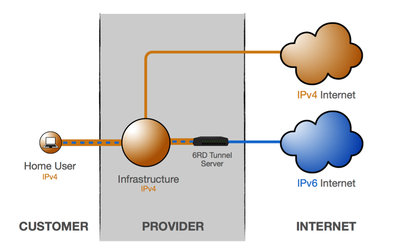
\includegraphics[width=\textwidth,height=\textheight,keepaspectratio]{6rd_1.png}
\centering
\caption{6rd visualisatie \autocite{RIPE2016}}
\centering
\end{figure}

Net zoals bij 6to4 moeten de IPv4-adressen van de tunneleindpunten in het IPv6-adres van de eindgebruiker worden geïntegreerd. Aangezien de eerste 32 bits van het IPv6-adres van het eindapparaat opgenomen zal worden door de prefix van de ISP en de tweede 32 bits gebruikt zal worden voor de IPv4 adressen van de tunneleindes. Slechts één /64 IPv6 range zal beschikbaar zijn voor elk apparaat \autocite{RIPE2016}.

\begin{figure}
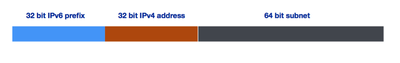
\includegraphics[width=\textwidth,height=\textheight,keepaspectratio]{6rd.png}
\centering
\caption{6rd schematische voorstelling deel 1 \autocite{RIPE2016}}
\centering
\end{figure}

Het aanvragen van een grotere toewijzing van adresruimte, /29 in plaats van een /32, zou drie extra bits betekenen. Dit komt overeen met acht IPv6-subnetten die aan elk eindapparaat kan toegewezen worden in plaats van slechts één \autocite{RIPE2016}. 

\begin{figure}
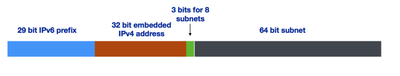
\includegraphics[width=\textwidth,height=\textheight,keepaspectratio]{6rd_2.png}
\centering
\caption{6rd schematische voorstelling deel 2 \autocite{RIPE2016}}
\centering
\end{figure}

Er is ook de mogelijkheid om te kiezen voor alleen het variabele deel van een IPv4-adres in het 6rd IPv6-adres te integreren. Als er een /21 IPv4-allocatie gebruikt wordt, dan betekent dat, dat de variabele bits, de laatste 11 bits, worden geïntegreerd in plaats van alle 32 bits van het IPv4-adres \autocite{RIPE2016}.

\begin{figure}
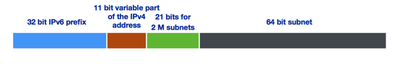
\includegraphics[width=\textwidth,height=\textheight,keepaspectratio]{6rd_3.png}
\centering
\caption{6rd schematische voorstelling deel 3 \autocite{RIPE2016}}
\centering
\end{figure}

Het combineren van beide methodes, zowel het gebruik maken van een /29 IPv6-toewijzing en het gebruik maken van de variabele bits van het IPv4 adres, geeft ons het volgende weer \autocite{RIPE2016}.

\begin{figure}
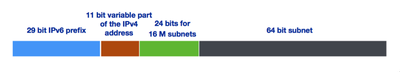
\includegraphics[width=\textwidth,height=\textheight,keepaspectratio]{6rd_4.png}
\centering
\caption{6rd schematische voorstelling deel 4 \autocite{RIPE2016}}
\centering
\end{figure}

\subsection{DS-Lite}

DS-Lite staat voor Dual Stack Lite en is vooral gebaseerd op native IPv6, tunneling en NAT (Network Address Translation).

In tegenstelling tot alle andere transitietechnieken die reeds besproken zijn, gaat DS-Lite zijn IPv4-pakketten inkapselen in IPv6-pakketten. Wat resulteert in het tunnelen van IPv4 over IPv6. Dit is precies de tegenovergestelde werking van alle vorige besproken methodes \autocite{RIPE2016}.

DS-Lite kan een IPv6-apparaat verbinding laten maken met een IPv4-apparaat en het IPv4-internet. Het voornaamste doel van DS-Lite is dat een ISP geen publiek IPv4 adres maar moet toewijzen aan een klant. In plaats daarvan worden alleen globale IPv6-adressen toegewezen \autocite{RIPE2016}.

De CPE verdeelt, hetzelfde als een NAT-apparaat, private IPv4-adressen aan klanten. In plaats van de NAT zelf laten uit te voeren gaat de CPE het IPv4-pakket inkapselen in een IPv6-pakket. De CPE maakt hierbij gebruik van zijn wereldwijde IPv6-verbinding om het pakket op een correcte manier af te leveren aan de CGN van de ISP (carrier-grade NAT) dat een openbaar IPv4-adres heeft. Het IPv6 pakket wordt op zijn beurt uitgepakt waardoor het IPv6 pakket terug naar het oorspronkelijke IPv4 pakket wordt hersteld. NAT zal nadien uitgevoerd worden op het IPv4-pakket en het pakket zal zo door het openbare IPv4-internet gestuurd worden naar zijn bestemming \autocite{RIPE2016}. 

\begin{figure}
\centering
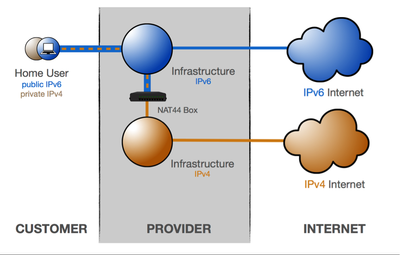
\includegraphics[width=\textwidth,height=\textheight,keepaspectratio]{dslite.png}
\caption{DS-Lite visualisatie \autocite{RIPE2016}}
\end{figure}

\subsection{Teredo}

Teredo is een per-host tunneltechniek voor het verzenden van IPv6 pakketten achter NAT apparaten via IPv4. De IPv6-pakketten worden ingepakt als een IPv4-pakket met een UDP header van het bestemmingsadres van een Teredo server met een welbekend UDP poort 3544. De algemene Teredo server voor windows is teredo.ipv6.microsoft.com. Alle tunnels naar Teredo gebruikers delen dezelfde IPv6 prefix namelijk 2001:0::/32 gevolgd door het IPv4 adres van de gebruikte Teredo Server. In het geval van Microsoft is dit 94.245.121.251 en omgezet in hexadecimaal is het 5ef5:79fb. Het adres met beide prefixen ziet er als volgt uit, 2001:0:5ef5:79fb::/64 \autocite{Vinciguerra2013}.

\begin{figure}
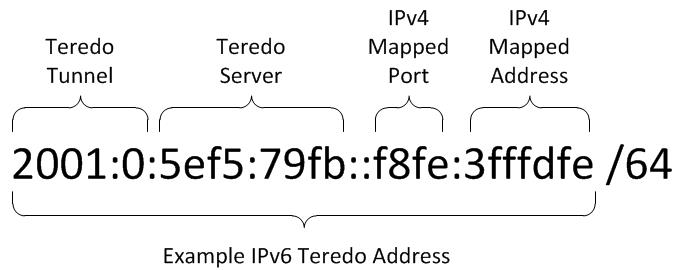
\includegraphics[width=\textwidth,height=\textheight,keepaspectratio]{teredo.jpg}
\centering
\caption{Teredo schematische voorstelling \autocite{Vinciguerra2013}}
\centering
\end{figure}

De Teredo gebruiker zal een IPv4 router soliciation versturen naar de Teredo server. Nadien zal de server de gebruiker voorzien van zijn IPv6-adres door het versleutelen van zijn IPv6-adres door het NATed bron IPv4-adres en de UDP-bronpoort naar het einde van het IPv6-adres \autocite{Vinciguerra2013}.

\begin{figure}
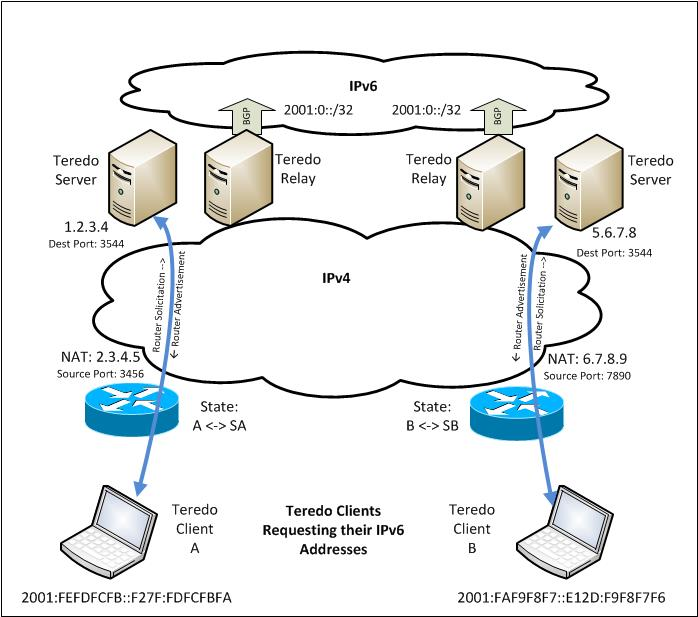
\includegraphics[width=\textwidth,height=\textheight,keepaspectratio]{teredo2.jpg}
\centering
\caption{Teredo visualisatie \autocite{Vinciguerra2013}}
\centering
\end{figure}

Het Teredo protocol is gebaseerd op een speciaal IPv6-pakket zonder payload dat een luchtbeld wordt genoemd, om door NAT apparaten te geraken. Er zijn twee soorten bubbels. Als eerst zijn er de directe bubbels, die van Teredo peer naar Teredo peer worden verstuurd. Als tweede zijn er de indirecte bubbels die door de Teredo server van de peer verstuurd worden \autocite{teredo}.

\subsection{ISATAP}

ISATAP (Intra Site Automatic Tunneling Address Protocol) is een interface die hosts kunnen gebruiken om IPv6 verkeer over een IPv4 netwerk te laten verzenden. Door het toevoegen van headers met IPv4 netwerk informatie aan het IPv6 pakket kan de gebruiker pakketten verzenden over het netwerk naar een IPv6 bestemming. Nadien kan de ontvanger van het pakket deze uitpakken tot zijn originele staat \autocite{RIPE2016}.

ISATAP is vrij eenvoudig om te herkennen. De adressen die dit protocol hanteert zijn zeer uniek geformatteerd. Een voorbeeld van een ISATAP adres is 2002:9D36:1:2:0:5EFE:192:168:12:9 \autocite{RIPE2016}.

Bij nader inzien zijn er twee opvallende delen aan het adres. Het eerste deel, 2002:9D36:1:2:0:5EFE: is geformatteerd als een typisch IPv6 adres. Het tweede deel, 192.168.12.9, is het formaat van een IPv4 adres. Het formaat hiervan bevat essentiële informatie. Ten eerste is het adres een geldig IPv6 adres waarmee IPv6 connectie mogelijk is. Vervolgens geeft de aanwezigheid van het IPv4-adres, de IPv4-informatie aan die zal gebruikt worden om het IPv6-verkeer over het IPv4-netwerk te leiden \autocite{RIPE2016}.

\begin{figure}
  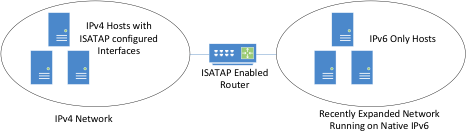
\includegraphics[width=\textwidth,height=\textheight,keepaspectratio]{isatap.png}
  \centering
  \caption{ISATAP visualisatie \autocite{RIPE2016}}
  \centering
\end{figure}

Met een ISATAP router en het configureren van ISATAP bij hosts in het IPv4 netwerk, is het mogelijk om IPv6 only hosts te laten communiceren met het IPv4 netwerk \autocite{RIPE2016}.

\section{Translatie}

In het geval van een translatie zal het pakket niet worden ingepakt als een IPv4 pakket. In dit geval zal de IPv6 header van het pakket vervangen worden door een IPv4 header. Hierdoor zal het IPv6 pakket vertaald en omgezet worden naar een IPv4. Enkele technieken die hiervoor worden uitgelegd zijn  NAT64/DNS64 en 464XLAT \autocite{RIPE2016}.

\subsection{NAT64/DNS64}

NAT64/DNS64 is een methode die het mogelijk maakt om voor IPv6 klanten connecties te laten maken naar IPv4-apparaten.

In het netwerk van de ISP is er een translator box aanwezig (NAT64 server) die de headers van een IPv6-pakket verwijderen en vervangen met een IPv4-header. De NAT64 server is het eindpunt voor op tenminste één IPv4 adres en een IPv6 netwerk segment van 32 bits \autocite{RIPE2016}.

Het meest centrale deel van dit mechanisme is DNS64. In het geval van DNS64 zet de DNS-server IPv6 DNS queries om naar IPv4 DNS queries. Achteraf zullen de ontvangen pakketten omgezet worden van IPv4 DNS records naar IPv6 records \autocite{RIPE2016}.

NAT64/DNS64 wordt hoofdzakelijk gebruikt bij grote mobiele providers.

\subsection{464XLAT}

Een mogelijk probleem bij sommige mobile apps is dat deze enkel IPv4 connecties ondersteunend zijn en dus niet functioneel zijn met IPv6.

Om dit probleem te verhelpen is een extra transitie methode nodig namelijk 464XLAT. Dit wordt in gebruikt in combinatie met NAT64/DNS64 \autocite{RIPE2016}.

464XLAT wordt geactiveerd via het installeren van software op het IPv6 mobiele apparaat, CLAT demon \autocite{RIPE2016}.

464XLAT zal het mobiele apparaat een dummy IPv4 geven. Op deze manier kunnen de applicaties die enkel IPv4 ondersteunen gebruik maken van deze dummy. Achteraf zal CLAT demon een lokale vertaling doen naar IPv6 op het apparaat \autocite{RIPE2016}.

\begin{figure}
\centering
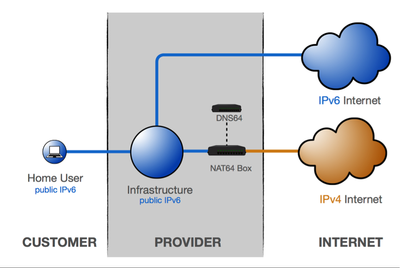
\includegraphics[width=\textwidth,height=\textheight,keepaspectratio]{nat64.png}
\caption{NAT64 visualisatie \autocite{RIPE2016}}
\end{figure}

\section{Besluit}

Bij het gebruiken van deze methodes komt er ook een extra complexiteit bij te pas. Dit zal het netwerk niet vergemakkelijken en hecht een zeker kennis en onderhoud van het netwerk. Deze methodes zouden op elk ogenblik vermeden moeten worden waar mogelijk. Een betere oplossing voor dit probleem zou het toepassen van DS-Lite kunnen zijn. Deze mechaniek heeft een lagere complexiteit en brengt minder nadelen met zich mee.